\section{CW attack}


\begin{frame}{CW attack}
    \begin{itemize}
        \item \textbf{Title:}Towards Evaluating the Robustness of Neural Networks
        \item \textbf{Author:} Nicholas Carlini, David Wagner\footnote{University of California, Berkeley}
        % \item \textbf{Contribution}
    \end{itemize}
\end{frame}

\begin{frame}{生成对抗样本的思路}
    CW攻击是一种基于优化的攻击方式,其攻击思路主要有
    \begin{itemize}
        \item 添加的扰动尽量小,$x+\delta \in [0,1]^n$
        \item 对抗样本和干净样本的距离越小越好,即$\text{minimize}\quad D(x,x+\delta)$
        \item 对抗样本应该使得模型分类错误$C(x+\delta)=t$,且分类错误的概率越高越好
    \end{itemize}

    对抗样本的公式:原始样本$x$和生成的对抗样本$x+\delta$之间的距离为$D(x,x+\delta)$,使得模型$C$在输入对抗样本$x+\delta$的情况下,产生错误的分类预测结果$t$。
    \begin{equation}
        \begin{aligned}
            \text{minimize}\quad    & D(x,x+\delta) \\
            \text{such that}\quad   & C(x+\delta)=t \\
                                    & x+\delta \in [0,1]^n
        \end{aligned}
        \label{L-BFGS}
    \end{equation}    
\end{frame}

\begin{frame}{构建对抗样本}
    但是由于$C$是高度非线性的,公式\ref{L-BFGS}很难求解,因此文中定义一个目标函数$f$,使得$C(x+\delta)=t$当且仅当$f(x+\delta)\leq 0$,上面的公式就可以变成
    \begin{equation}
        \begin{aligned}
            \text{minimize}\quad    & D(x,x+\delta)+c\cdot f(x+\delta) \\
            \text{such that}\quad   & C(x+\delta)=t \\
                                    & x+\delta \in [0,1]^n
        \end{aligned}
    \end{equation}
    $c$是一个超参数,并且$c>0$。
\end{frame}


\begin{frame}{构建对抗样本}
    \begin{multicols}{2}
        \begin{figure}
            \centering
            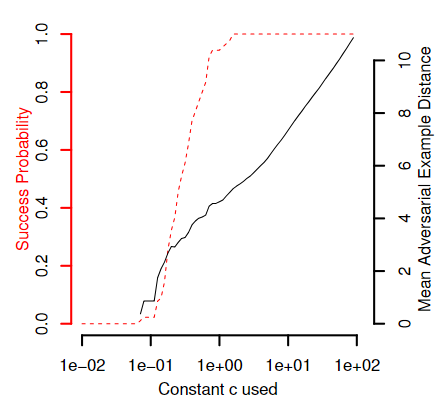
\includegraphics[width=0.4\textwidth]{docs/paperReading/CW_attack/const-c.png}
        \end{figure}
        实验发现,随着参数$c$的增大,攻击成功率(左侧红色虚线)和对抗样本平均距离(也就是对抗扰动,右侧黑色实线)也都会增大。在$c=0.1$附近的取值能够使得攻击成功率较小的情况下,扰动也较小
    \end{multicols}
\end{frame}


\begin{frame}{构建对抗样本}    
    需要对扰动$\delta_i$添加一个约束(论文中称为 Box constraints),$0\leq x_i+\delta_i\leq 1$

    引入参数$\omega_i$,假定
    \begin{equation}
        -1\leq \tanh(\omega_i)\leq 1
    \end{equation}
    那么
    \begin{equation}
        0\leq \frac{1}{2}(\tanh(\omega_i)+1)\leq 1
    \end{equation}
    可以得到CW方法中对$\delta_i$的约束
    \begin{equation}
        x_i+\delta_i=\frac{1}{2}(\tanh(\omega_i)+1)
    \end{equation}
    公式就可以改写成
    \begin{equation}
        \begin{aligned}
            \text{minimize}\quad    & D(x,x+\delta)+c\cdot f(\frac{1}{2}(\tanh(\omega_i)+1)) \\
            \text{such that}\quad   & C(x+\delta)=t \\
                                    & x+\delta \in [0,1]^n
        \end{aligned}
    \end{equation}

\end{frame}


\begin{frame}{构建对抗样本}
    对于公式中的$f$
    \begin{equation}
        \begin{aligned}
            f_1(x') & = -loss_{F,t}(x')+1 \\
            f_2(x') & = [\mathop{\max}\limits_{i\neq t}(F(x')_i)-F(x')_t]^+ \\
            f_3(x') & = \text{softplus}[\mathop{\max}\limits_{i\neq t}(F(x')_i)-F(x')_t]-\log(2) \\
            f_4(x') & = (0.5-F(x')_t)^+ \\
            f_5(x') & = -\log(2F(x')_t-2)^+ \\
            f_6(x') & = [\mathop{\max}\limits_{i\neq t}(Z(x')_i)-Z(x')_t]^+ \\
            f_7(x') & = \text{softplus}[\mathop{\max}\limits_{i\neq t}(Z(x')_i)-Z(x')_t]-\log(2)
        \end{aligned}
    \end{equation}
    其中$(e)^+=max(e,0)$,$\text{softplus}(x)=\log(1+e^x)$,$\text{loss}_{F,s}(x)$是$x$的交叉熵损失
\end{frame}


\begin{frame}{构建对抗样本}
    \begin{scriptsize}
        距离$D(x,x+\delta)$的计算可以选择$L_1,L_2,L_\infty$三种
        \begin{itemize}
            \item $L_2$ 攻击
        \end{itemize}
        \begin{equation}
            \begin{aligned}
                \text{minimize}\quad ||\frac{1}{2}(\tanh(\omega)+1)-x||_2^2+c\cdot f(\frac{1}{2}(\tanh(\omega_i)+1)) \\
                f(x')=\max(\max\left\{Z(x')_i:i\neq t\right\}-Z(x')_t,-\kappa),\quad set \kappa=0
            \end{aligned}
        \end{equation}


        \begin{itemize}
            \item $L_0$ 攻击
        \end{itemize}
        $L_0$距离度量是不可微的,因此不适合标准梯度下降。作者使用迭代算法,在每次迭代中,识别对输出结果没有太大影响的像素,并且固定其数值不做修改。

        \begin{itemize}
            \item $L_\infty$ 攻击
        \end{itemize}
        $L_\infty$距离度量效果并不好,作者使用了迭代攻击来解决这个问题
        \begin{equation}
            \text{minimize}\quad \sum[(\delta_i-\tau)^+]+c\cdot f(\frac{1}{2}(\tanh(\omega_i)+1))
        \end{equation}
        $(\delta_i-\tau)^+=\max(\delta_i-\tau,0)$,惩罚任何超过$\tau$的扰动$\delta_i$,$0.9\leq \tau\leq 1$,\(\tau\)从1开始减小,小于0.9时停止
    \end{scriptsize}
\end{frame}

\begin{frame}{实验}
    三种范数下的CW攻击(MNIST数据集)结果
    \begin{figure}
        \centering
        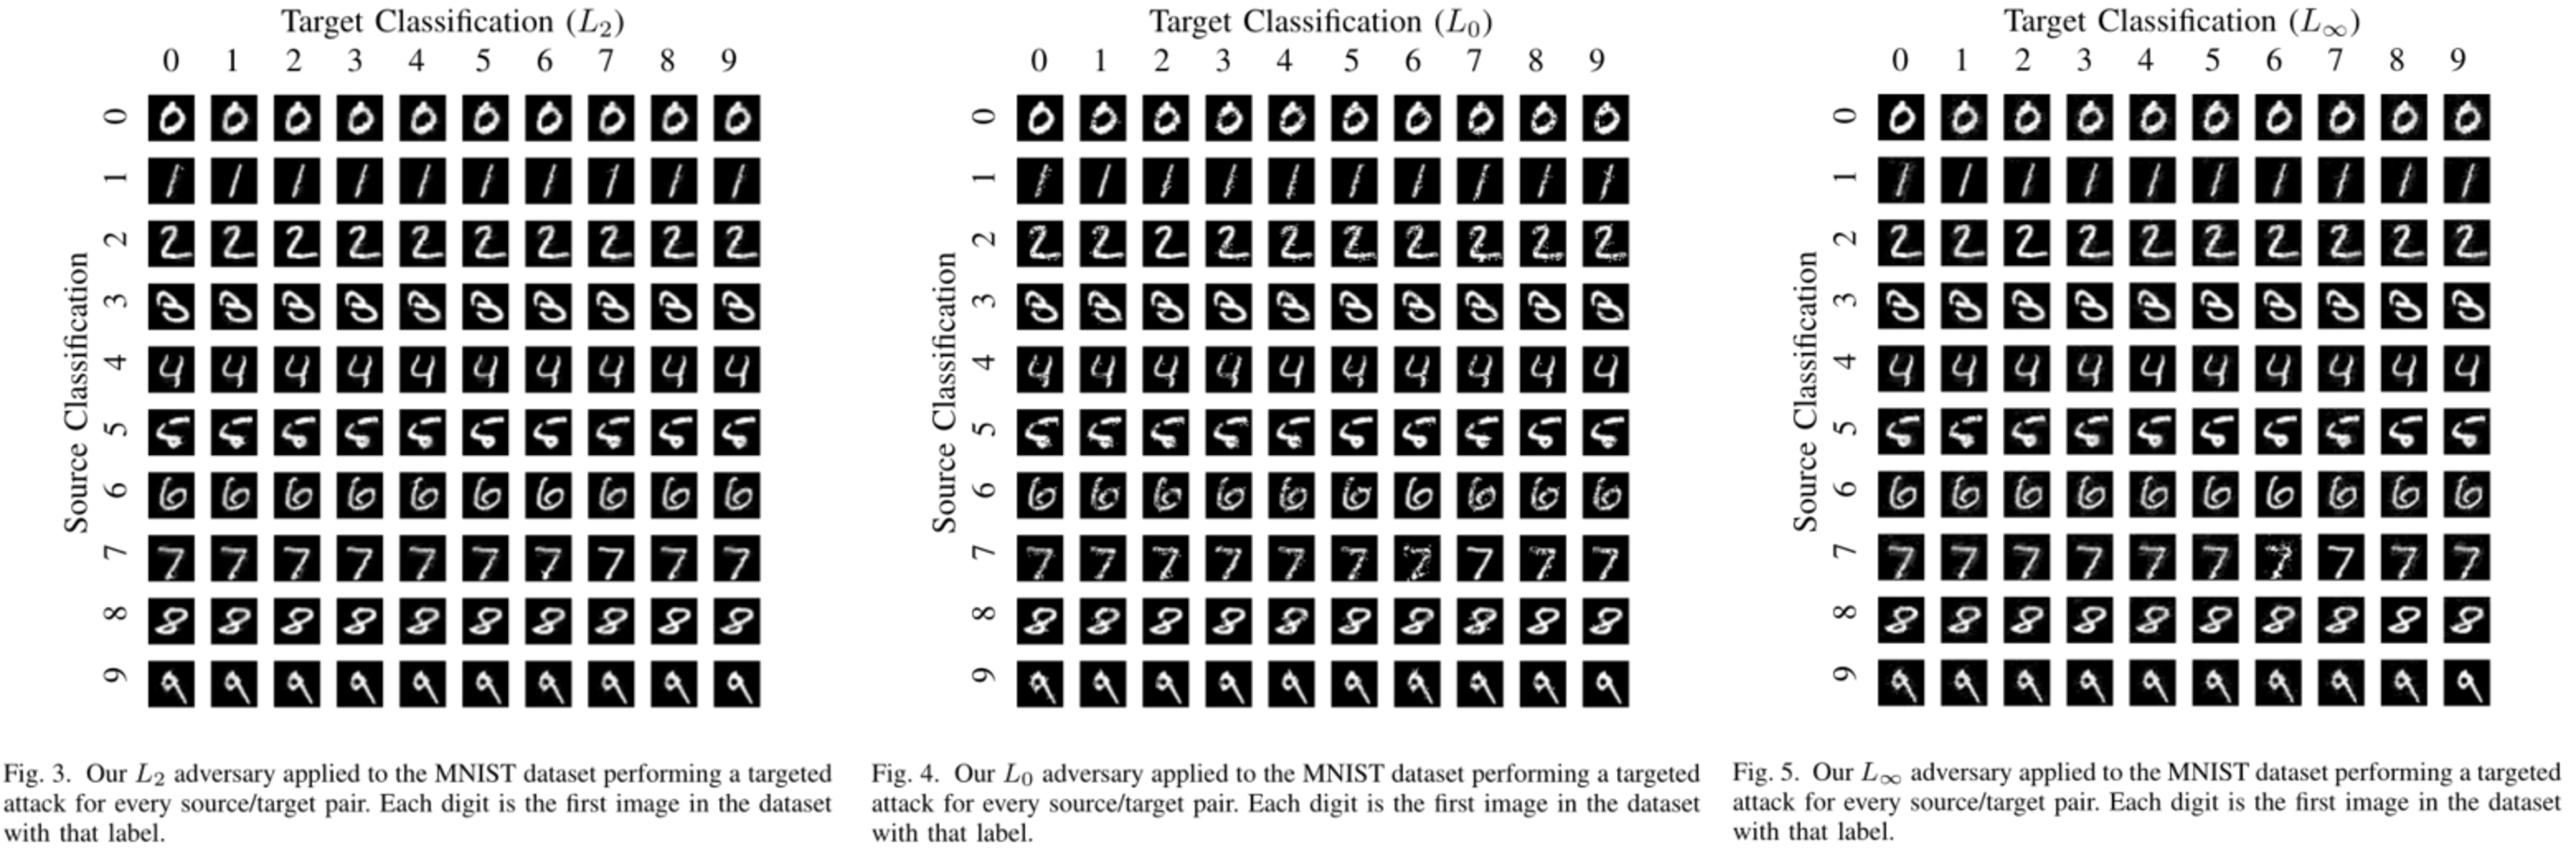
\includegraphics[width=1.0\textwidth]{docs/paperReading/CW_attack/attack-sample.png}
    \end{figure}
\end{frame}


\begin{frame}{实验}
    CW的攻击扰动都很小
    \begin{figure}
        \centering
        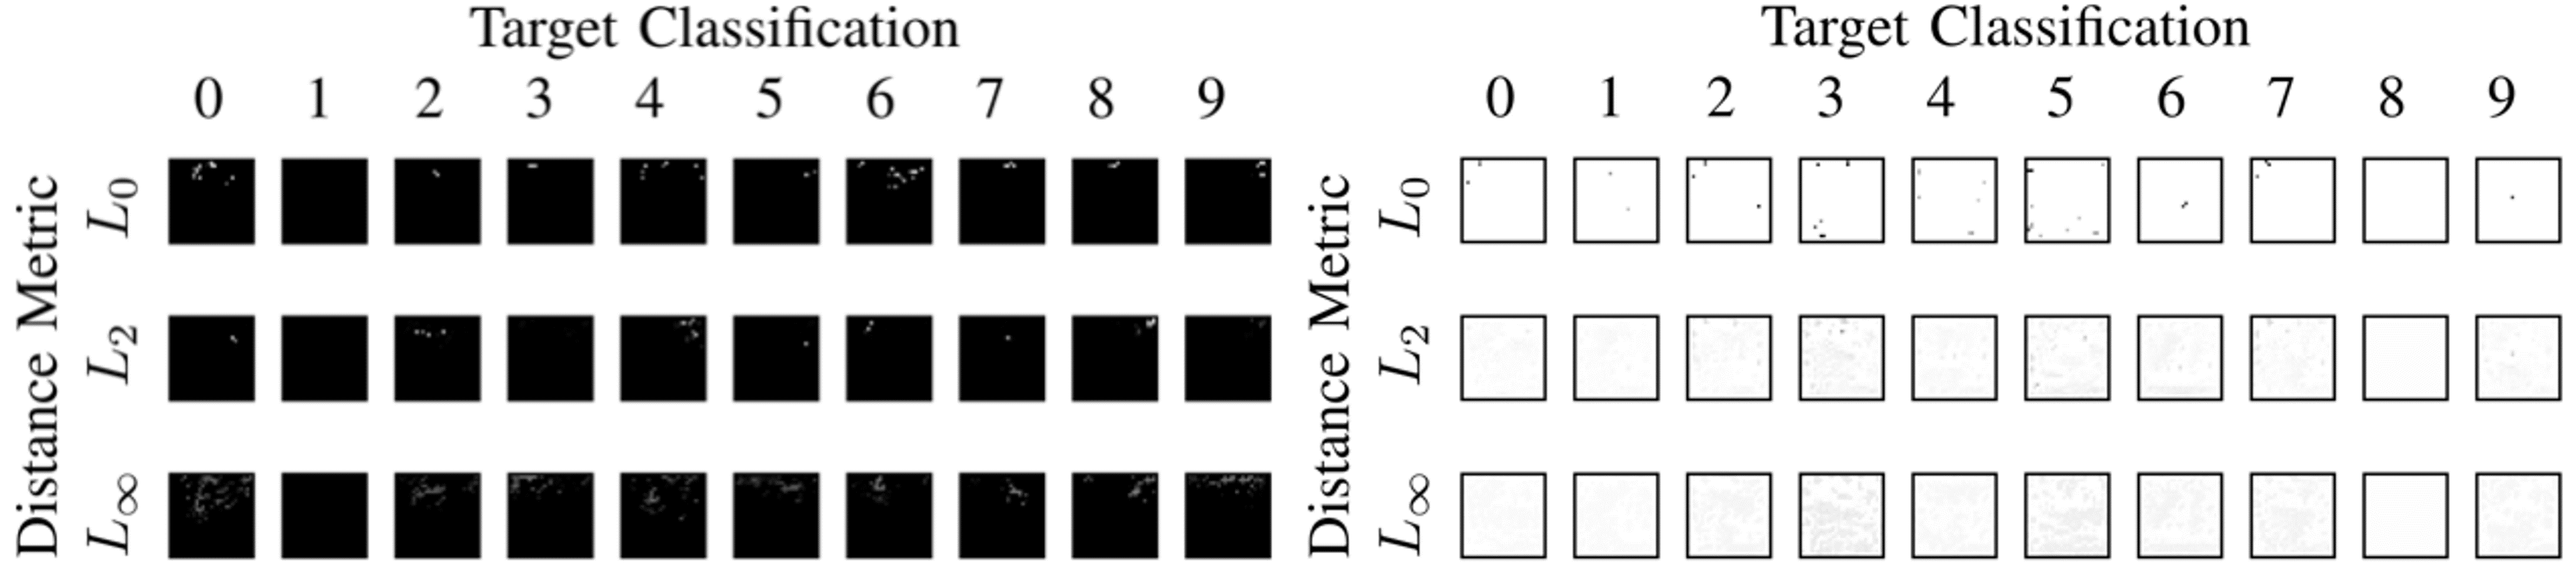
\includegraphics[width=1.0\textwidth]{docs/paperReading/CW_attack/per.png}
    \end{figure}
\end{frame}

\begin{frame}{实验}
    作者对ImageNet进行攻击,攻击扰动也很小
    \begin{figure}
        \centering
        \includegraphics[width=0.9\textwidth]{docs/paperReading/CW_attack/imagenet.png}
    \end{figure}
\end{frame}

\begin{frame}{实验}
    $L_2$的攻击扰动小,但是攻击的速度很慢
    \begin{figure}
        \centering
        \includegraphics[width=1.05\textwidth]{docs/paperReading/CW_attack/cw-exp.png}
    \end{figure}    
\end{frame}